% Options for packages loaded elsewhere
\PassOptionsToPackage{unicode}{hyperref}
\PassOptionsToPackage{hyphens}{url}
\documentclass[
]{article}
\usepackage{xcolor}
\usepackage[margin=1in]{geometry}
\usepackage{amsmath,amssymb}
\setcounter{secnumdepth}{-\maxdimen} % remove section numbering
\usepackage{iftex}
\ifPDFTeX
  \usepackage[T1]{fontenc}
  \usepackage[utf8]{inputenc}
  \usepackage{textcomp} % provide euro and other symbols
\else % if luatex or xetex
  \usepackage{unicode-math} % this also loads fontspec
  \defaultfontfeatures{Scale=MatchLowercase}
  \defaultfontfeatures[\rmfamily]{Ligatures=TeX,Scale=1}
\fi
\usepackage{lmodern}
\ifPDFTeX\else
  % xetex/luatex font selection
  \setmainfont[]{DejaVu Serif}
  \setsansfont[]{DejaVu Sans}
  \setmonofont[]{DejaVu Sans Mono}
\fi
% Use upquote if available, for straight quotes in verbatim environments
\IfFileExists{upquote.sty}{\usepackage{upquote}}{}
\IfFileExists{microtype.sty}{% use microtype if available
  \usepackage[]{microtype}
  \UseMicrotypeSet[protrusion]{basicmath} % disable protrusion for tt fonts
}{}
\makeatletter
\@ifundefined{KOMAClassName}{% if non-KOMA class
  \IfFileExists{parskip.sty}{%
    \usepackage{parskip}
  }{% else
    \setlength{\parindent}{0pt}
    \setlength{\parskip}{6pt plus 2pt minus 1pt}}
}{% if KOMA class
  \KOMAoptions{parskip=half}}
\makeatother
\usepackage{longtable,booktabs,array}
\usepackage{calc} % for calculating minipage widths
% Correct order of tables after \paragraph or \subparagraph
\usepackage{etoolbox}
\makeatletter
\patchcmd\longtable{\par}{\if@noskipsec\mbox{}\fi\par}{}{}
\makeatother
% Allow footnotes in longtable head/foot
\IfFileExists{footnotehyper.sty}{\usepackage{footnotehyper}}{\usepackage{footnote}}
\makesavenoteenv{longtable}
\usepackage{graphicx}
\makeatletter
\newsavebox\pandoc@box
\newcommand*\pandocbounded[1]{% scales image to fit in text height/width
  \sbox\pandoc@box{#1}%
  \Gscale@div\@tempa{\textheight}{\dimexpr\ht\pandoc@box+\dp\pandoc@box\relax}%
  \Gscale@div\@tempb{\linewidth}{\wd\pandoc@box}%
  \ifdim\@tempb\p@<\@tempa\p@\let\@tempa\@tempb\fi% select the smaller of both
  \ifdim\@tempa\p@<\p@\scalebox{\@tempa}{\usebox\pandoc@box}%
  \else\usebox{\pandoc@box}%
  \fi%
}
% Set default figure placement to htbp
\def\fps@figure{htbp}
\makeatother
\setlength{\emergencystretch}{3em} % prevent overfull lines
\providecommand{\tightlist}{%
  \setlength{\itemsep}{0pt}\setlength{\parskip}{0pt}}
% UTF-8 and font configuration for LuaLaTeX
\usepackage{fontspec}
\defaultfontfeatures{Ligatures=TeX,Scale=MatchLowercase}

% Link handling and pdf metadata hooks
\usepackage{hyperref}

\usepackage{enumitem}
\usepackage{amssymb}
\setlistdepth{9}
\renewlist{itemize}{itemize}{9}
\setlist[itemize]{label=\textbullet}
\setlist[itemize,1]{label=\textbullet}
\setlist[itemize,2]{label=\textendash}
\setlist[itemize,3]{label=\textasteriskcentered}
\setlist[itemize,4]{label=\textperiodcentered}
\setlist[itemize,5]{label=\diamond}
\setlist[itemize,6]{label=\circ}
\setlist[itemize,7]{label=\triangleright}
\setlist[itemize,8]{label=\triangleleft}
\setlist[itemize,9]{label=\square}
\title{\texorpdfstring{The ERDA Book}{The ERDA Book}}\author{}\date{}\AtBeginDocument{\maketitle}
\newcommand{\fallbackfeature}{}
\directlua{local fonts={"Twemoji Mozilla:mode=harf", "ERDA CC-BY CJK:mode=harf", "DejaVu Sans:mode=harf"}; local filtered={}; local function gbw_nonempty_table(t) return type(t) == 'table' and next(t) ~= nil end; for _, name in ipairs(fonts) do   local base = tostring(name):match('^([^:]+)') or name;   local ok1, info = pcall(function() return luaotfload.aux.provides_font(base) end);   if ok1 and type(info) == 'table' and info.filename then     table.insert(filtered, base);   else     texio.write_nl('log', 'luaotfload fallback skipped missing font: '..tostring(base));   end; end; gbw_fallback_stack = filtered; texio.write_nl('log', 'luaotfload fallback filtered='..table.concat(filtered, '; ')); if not gbw_nonempty_table(filtered) then   texio.write_nl('log', 'luaotfload fallback list empty; skipping add_fallback'); else   local ok2, err = pcall(function() luaotfload.add_fallback("mainfont", filtered) end);   if not ok2 then     texio.write_nl('log', 'luaotfload.add_fallback skipped: '..tostring(err));   else     local fb = luaotfload and luaotfload.fallbacks and luaotfload.fallbacks["mainfont"];     if gbw_nonempty_table(fb) then       if token and token.set_macro then token.set_macro('fallbackfeature', 'RawFeature={fallback=mainfont}', true); else texio.write_nl('log', 'gbw: token.set_macro unavailable; cannot set fallbackfeature'); end;     else       texio.write_nl('log', 'luaotfload.add_fallback produced empty data; skipping fallbackfeature');     end;   end; end}
\directlua{texio.write_nl('term and log', '*** GBW: Missing glyph detector initialized (abort=false)');gbw_missing_glyphs = gbw_missing_glyphs or {};local function gbw_font_name(fid)  local f = font.getfont(fid);  if not f then return tostring(fid) end;  return f.fullname or f.psname or f.name or tostring(fid);end;local function gbw_note_missing(fid, cp)  local entry = gbw_missing_glyphs[cp];  if not entry then entry = {fonts={}}; gbw_missing_glyphs[cp]=entry end;  entry.fonts[gbw_font_name(fid)] = true;  texio.write_nl('term and log', '*** GBW: Noted missing glyph U+'..string.format('%04X', cp)..' in font '..gbw_font_name(fid));end;local function gbw_check(head)  for n in node.traverse_id(node.id('glyph'), head) do    local fid = n.font; local cp = n.char;    if fid and cp then      local ok, has = pcall(font.has_glyph, fid, cp);      if (not ok) or (not has) then gbw_note_missing(fid, cp) end;    end  end;  return head;end;local function gbw_report()  texio.write_nl('term and log', '*** GBW: gbw_report() called');  if not gbw_missing_glyphs then texio.write_nl('term and log', '*** GBW: gbw_missing_glyphs is nil'); return end;  local keys = {}; for cp,_ in pairs(gbw_missing_glyphs) do keys[#keys+1]=cp end;  table.sort(keys);  texio.write_nl('term and log', '*** GBW: Found '..#keys..' missing glyph codepoints');  if #keys==0 then return end;  texio.write_nl('log', 'gbw missing glyph report ('..#keys..' codepoints)');  local fb = gbw_fallback_stack;  if type(fb) == 'table' and next(fb) ~= nil then     local okc, fb_str = pcall(function() return table.concat(fb, '; ') end);    if okc and fb_str then texio.write_nl('log', '  fallback stack: '..fb_str) end;  end;  local summary_lines = {};  for _,cp in ipairs(keys) do    local entry = gbw_missing_glyphs[cp];    local fonts = {}; for name,_ in pairs(entry.fonts or {}) do fonts[#fonts+1]=name end; table.sort(fonts);    local char_repr = ''; local ok,ch = pcall(function() return unicode.utf8.char(cp) end);    if ok and ch then char_repr = ' \"'..ch..'\"' end;    local line = string.format('  U+%04X%s missing in fonts: %s', cp, char_repr, table.concat(fonts, ', '));    texio.write_nl('log', line); summary_lines[#summary_lines+1]=line;  end;  if false then    texio.write_nl('term and log', '*** GBW: Aborting due to missing glyphs');    io.stderr:write('\\n=== GBW MISSING GLYPH ERROR ===\\n');    io.stderr:write('Found '..#keys..' codepoints with missing glyphs after fallback\\n');    if type(fb) == 'table' and next(fb) ~= nil then io.stderr:write('Fallback stack: '..table.concat(fb, '; ')..'\\n') end;    for _,l in ipairs(summary_lines) do io.stderr:write(l..'\\n') end;    io.stderr:write('=================================\\n');    io.stderr:flush();    tex.error('Missing glyphs after fallback', table.concat(summary_lines, '\\n'));  end;end;local lb = luatexbase or require('luatexbase');if lb and lb.add_to_callback then  texio.write_nl('term and log', '*** GBW: Registering callbacks');  lb.add_to_callback('hpack_filter', gbw_check, 'gbw-missing-glyphs-h');  lb.add_to_callback('pre_linebreak_filter', gbw_check, 'gbw-missing-glyphs-v');  lb.add_to_callback('finish_pdffile', gbw_report, 'gbw-missing-glyphs-report');  texio.write_nl('term and log', '*** GBW: Callbacks registered successfully');else  texio.write_nl('term and log', 'gbw missing glyph detector: luatexbase unavailable; skipping');end;}
\setmainfont[\fallbackfeature]{DejaVu Serif}
\setsansfont[\fallbackfeature]{DejaVu Sans}
\setmonofont[\fallbackfeature]{DejaVu Sans Mono}
\usepackage{bookmark}
\IfFileExists{xurl.sty}{\usepackage{xurl}}{} % add URL line breaks if available
\urlstyle{same}
\hypersetup{
  pdftitle={Template for multilingual neutral text},
  pdfauthor={ERDA Team},
  hidelinks,
  pdfcreator={LaTeX via pandoc}}

\title{Template for multilingual neutral text}
\author{ERDA Team}
\date{2024-06-02}

\begin{document}
\maketitle

{
\setcounter{tocdepth}{3}
\tableofcontents
}
\ifnum0\ifdefined\directlua\directlua{
    if ("\luaescapestring{\luatexbanner}"):match("LuaHBTeX") then tex.write("1") end
  }\fi>0 % LuaHBTeX is ok
  \setfontface\panEmojiFont{Twemoji Mozilla}[Renderer=HarfBuzz]
\else
  \PackageError{latex-emoji}{You must install a new TeX system (TeX Live 2020)\MessageBreak
    and then use 'lualatex' engine to print emoji}
   {The compilation will be aborted.}
  \let\panEmojiFont\relax
\fi
\ifdefined\ltjdefcharrange
\ltjdefcharrange{208}{
"200D,
"23F0,
"23F1,
"23F2,
"2600,
"2615,
"2618,
"261D,
"262A,
"262E,
"262F,
"2640,
"2642,
"265F,
"267B,
"2695,
"2697,
"2699,
"26A0,
"26A7,
"26BD,
"26BE,
"26C5,
"26C8,
"26D4,
"26F3,
"26F4,
"26F7,
"26F8,
"2708,
"270B,
"270D,
"271D,
"2721,
"2755,
"2757,
"2B50,
"FE0F,
"1F1E6,
"1F1E7,
"1F1E8,
"1F1E9,
"1F1EA,
"1F1EB,
"1F1EC,
"1F1EE,
"1F1EF,
"1F1F0,
"1F1F1,
"1F1F3,
"1F1F5,
"1F1F7,
"1F1F8,
"1F1F9,
"1F1FA,
"1F1FF,
"1F300,
"1F308,
"1F30C,
"1F30D,
"1F30E,
"1F30F,
"1F310,
"1F319,
"1F320,
"1F324,
"1F327,
"1F329,
"1F32A,
"1F32B,
"1F331,
"1F333,
"1F335,
"1F33D,
"1F33E,
"1F33F,
"1F340,
"1F347,
"1F34A,
"1F34C,
"1F34D,
"1F34E,
"1F353,
"1F35A,
"1F35D,
"1F35E,
"1F369,
"1F36A,
"1F36B,
"1F370,
"1F375,
"1F376,
"1F377,
"1F37A,
"1F37F,
"1F39E,
"1F3A4,
"1F3A7,
"1F3A8,
"1F3AC,
"1F3AE,
"1F3AF,
"1F3B2,
"1F3B8,
"1F3B9,
"1F3BB,
"1F3C0,
"1F3C1,
"1F3C2,
"1F3C3,
"1F3C5,
"1F3C6,
"1F3C8,
"1F3CA,
"1F3D0,
"1F3D1,
"1F3D3,
"1F3EB,
"1F3F3,
"1F3F4,
"1F3F8,
"1F3FB,
"1F3FD,
"1F3FF,
"1F40D,
"1F419,
"1F41C,
"1F41D,
"1F41E,
"1F41F,
"1F420,
"1F421,
"1F422,
"1F426,
"1F427,
"1F42C,
"1F42D,
"1F430,
"1F431,
"1F433,
"1F436,
"1F438,
"1F439,
"1F43B,
"1F446,
"1F447,
"1F448,
"1F449,
"1F44D,
"1F44E,
"1F44F,
"1F450,
"1F466,
"1F467,
"1F468,
"1F469,
"1F46E,
"1F4A1,
"1F4A7,
"1F4BB,
"1F4D0,
"1F4DA,
"1F4DE,
"1F4E0,
"1F4E1,
"1F4F1,
"1F4F2,
"1F4F8,
"1F50B,
"1F50C,
"1F525,
"1F526,
"1F527,
"1F529,
"1F52C,
"1F52D,
"1F549,
"1F570,
"1F58C,
"1F5A5,
"1F5A8,
"1F5BC,
"1F5D3,
"1F5FA,
"1F600,
"1F601,
"1F603,
"1F604,
"1F605,
"1F606,
"1F60A,
"1F60D,
"1F610,
"1F611,
"1F618,
"1F622,
"1F628,
"1F62D,
"1F62E,
"1F62F,
"1F630,
"1F631,
"1F632,
"1F634,
"1F636,
"1F637,
"1F63B,
"1F642,
"1F645,
"1F64C,
"1F680,
"1F681,
"1F686,
"1F687,
"1F688,
"1F689,
"1F68A,
"1F68C,
"1F68E,
"1F692,
"1F697,
"1F699,
"1F69A,
"1F69B,
"1F69C,
"1F6A2,
"1F6A4,
"1F6AB,
"1F6B4,
"1F6B8,
"1F6E0,
"1F6E3,
"1F6E4,
"1F6E9,
"1F6EB,
"1F6EC,
"1F6F0,
"1F6F3,
"1F6F6,
"1F6F7,
"1F7E5,
"1F7E6,
"1F7E7,
"1F7E8,
"1F7E9,
"1F912,
"1F914,
"1F915,
"1F918,
"1F919,
"1F91D,
"1F91F,
"1F927,
"1F928,
"1F929,
"1F932,
"1F93A,
"1F941,
"1F947,
"1F948,
"1F949,
"1F94C,
"1F94E,
"1F950,
"1F954,
"1F955,
"1F95D,
"1F964,
"1F966,
"1F968,
"1F96F,
"1F970,
"1F973,
"1F985,
"1F98A,
"1F98B,
"1F98E,
"1F99C,
"1F99F,
"1F9A2,
"1F9AF,
"1F9B0,
"1F9B1,
"1F9B3,
"1F9BD,
"1F9C1,
"1F9C3,
"1F9C4,
"1F9C5,
"1F9D1,
"1F9D4,
"1F9D5,
"1F9E0,
"1F9E9,
"1F9EA,
"1F9EB,
"1F9EC,
"1F9ED,
"1F9F9,
"1F9FA,
"1F9FC,
"1FA9B,
"1FA9F,
"1FAA3,
"1FAA8}
\ltjsetparameter{jacharrange={-208}}
\fi
\newcommand*{\panEmoji}[1]{{\panEmojiFont#1}}

\# content

This folder contains the British English version of the neutral sample
book. Use \hyperref[md-index]{index.md} as the starting point.

If you add or rename pages, update \hyperref[md-summary]{SUMMARY.md}
accordingly.

\newpage

\# appendices

\newpage

\section{Appendix A -- Data sources and table
layout}\label{appendix-a-data-sources-and-table-layout}

\subsection{A.1 Data sources}\label{a.1-data-sources}

\begin{enumerate}
\def\labelenumi{\arabic{enumi}.}
\tightlist
\item
  Public climate data catalogues from regional weather services.
\item
  Neutral example values from internal sandbox systems.
\item
  International open-data repositories such as
  \href{https://data.un.org/}{UN Data} or
  \href{https://data.worldbank.org/}{World Bank Open Data}.
\end{enumerate}

\subsection{A.2 Table layout}\label{a.2-table-layout}

\textbar{} Column \textbar{} Data type \textbar{} Description \textbar{}
\textbar--------\textbar----------\textbar-------------\textbar{}
\textbar{} \texttt{timestamp} \textbar{} ISO-8601 \textbar{} Timestamp
of the measurement \textbar{} \textbar{} \texttt{metric} \textbar{}
String \textbar{} Measurement (temperature, humidity, etc.) \textbar{}
\textbar{} \texttt{value} \textbar{} Decimal number \textbar{} Measured
value \textbar{} \textbar{} \texttt{unit} \textbar{} String \textbar{}
Associated unit \textbar{} \textbar{} \texttt{notes} \textbar{} Free
text \textbar{} Context or notes \textbar{}

\subsection{A.3 Reuse}\label{a.3-reuse}

\begin{itemize}
\tightlist
\item
  The table can be imported directly into dataframes.
\item
  Use relative links such as \hyperref[md-chapters-chapter-02]{Chapter
  2} for cross-references.
\item
  Graphics can be found in the
  \href{../images/}{\texttt{content/.github/assets}} directory.
\end{itemize}

\newpage

\section{Appendix -- Emoji \& font
coverage}\label{appendix-emoji-font-coverage}

This overview summarises the fonts that cover all writing systems used
in the sample texts as well as all emoji sets. All fonts meet the
licensing requirements from \texttt{AGENTS.md} and the
\texttt{LICENSE-FONTS} file.

\subsection{Font matrix}\label{font-matrix}

\begin{longtable}[]{@{}
  >{\raggedright\arraybackslash}p{(\linewidth - 8\tabcolsep) * \real{0.2000}}
  >{\raggedright\arraybackslash}p{(\linewidth - 8\tabcolsep) * \real{0.2000}}
  >{\raggedright\arraybackslash}p{(\linewidth - 8\tabcolsep) * \real{0.2000}}
  >{\raggedright\arraybackslash}p{(\linewidth - 8\tabcolsep) * \real{0.2000}}
  >{\raggedright\arraybackslash}p{(\linewidth - 8\tabcolsep) * \real{0.2000}}@{}}
\toprule\noalign{}
\begin{minipage}[b]{\linewidth}\raggedright
Category
\end{minipage} & \begin{minipage}[b]{\linewidth}\raggedright
Font
\end{minipage} & \begin{minipage}[b]{\linewidth}\raggedright
Licence
\end{minipage} & \begin{minipage}[b]{\linewidth}\raggedright
Source
\end{minipage} & \begin{minipage}[b]{\linewidth}\raggedright
Coverage
\end{minipage} \\
\midrule\noalign{}
\endhead
\bottomrule\noalign{}
\endlastfoot
Serif/Sans/Mono & DejaVu Serif · DejaVu Sans · DejaVu Sans Mono (v2.37)
& Bitstream Vera License + public-domain additions &
\texttt{gitbook\_worker/defaults/fonts.yml} ·
\texttt{publish/ATTRIBUTION.md} & Latin, Greek, Cyrillic, plus technical
symbols for tables and code \\
CJK \& additional BMP glyphs & ERDA CC-BY CJK & CC BY 4.0 \textbf{or}
MIT & \texttt{.github/fonts/erda-ccby-cjk} · \texttt{LICENSE-FONTS} &
Chinese, Japanese, Korean, plus additional Unicode blocks from the
multilingual templates \\
Coloured emojis & Twemoji Color Font v15.1.0 & CC BY 4.0 &
https://github.com/13rac1/twemoji-color-font/releases/tag/v15.1.0 ·
\texttt{publish/ATTRIBUTION.md} & All emoji categories including skin
tones, ZWJ sequences and flags \\
\end{longtable}

\subsection{Practical use}\label{practical-use}

\begin{enumerate}
\def\labelenumi{\arabic{enumi}.}
\tightlist
\item
  \textbf{Text sections} -- The DejaVu family serves as the standard for
  body text (\texttt{SERIF}), UI elements (\texttt{SANS}) and code
  (\texttt{MONO}). This covers all European languages in
  \texttt{content/templates/multilingual-neutral-text.md}.
\item
  \textbf{CJK} -- As soon as chapters or example pages use characters
  such as 日, 学 or 정보, the build system should embed the
  ERDA-CC-BY-CJK file from
  \texttt{.github/fonts/erda-ccby-cjk/true-type/}. This happens
  automatically via the \texttt{CJK} section in
  \texttt{gitbook\_worker/defaults/fonts.yml}.
\item
  \textbf{Emoji colour} -- The new emoji example pages use the Twemoji
  colour font. \texttt{gitbook\_worker/defaults/fonts.yml} references
  the download URL so CI builds can fetch the TTF automatically.
\end{enumerate}

\subsection{Testing notes}\label{testing-notes}

\begin{itemize}
\tightlist
\item
  Run \texttt{pytest\ -k\ emoji} to ensure the font scanning does not
  report unknown fonts.
\item
  Check PDF exports with at least one page from each emoji category
  (smileys, nature, activities, objects) to test Twemoji alongside CJK
  text.
\item
  Document any new fonts in \texttt{publish/ATTRIBUTION.md} and
  \texttt{LICENSE-FONTS} if additional writing systems are added.
\end{itemize}

\newpage

\# chapters

\newpage

\section{Chapter 1 -- Observable
patterns}\label{chapter-1-observable-patterns}

This chapter introduces a neutral description of structured
observations. All examples are based on generic measurement points that
can be easily transferred to new contexts.

\subsection{1.1 Method steps}\label{method-steps}

\begin{enumerate}
\def\labelenumi{\arabic{enumi}.}
\tightlist
\item
  \textbf{Define the frame:} determine the purpose of the observation
  (e.g.~temperature, usage behaviour or process duration).
\item
  \textbf{Choose measurement points:} define neutral parameters that do
  not contain personal data.
\item
  \textbf{Secure documentation:} record measurement results in tables
  and cite the source, e.g.~public data catalogues.\footnote{See
    \hyperref[md-references]{Citations \& further reading}.}
\end{enumerate}

\subsection{1.2 Example description}\label{example-description}

\begin{itemize}
\tightlist
\item
  \emph{Measurement area:} a fictitious test area with a moderate
  climate.
\item
  \emph{Instruments:} standardised sensors with a calibration
  certificate.
\item
  \emph{Evaluation:} averages over a four-week period.
\end{itemize}

The resulting data is presented later in the book -- in particular in
\hyperref[md-chapters-chapter-02]{Chapter 2} -- in table form. Detailed
data is also provided in \hyperref[md-appendices-appendix-a]{Appendix
A}.

\subsection{1.3 Cross-references}\label{cross-references}

\begin{longtable}[]{@{}
  >{\raggedright\arraybackslash}p{(\linewidth - 4\tabcolsep) * \real{0.4583}}
  >{\raggedright\arraybackslash}p{(\linewidth - 4\tabcolsep) * \real{0.2917}}
  >{\raggedright\arraybackslash}p{(\linewidth - 4\tabcolsep) * \real{0.2500}}@{}}
\toprule\noalign{}
\begin{minipage}[b]{\linewidth}\raggedright
Section
\end{minipage} & \begin{minipage}[b]{\linewidth}\raggedright
Purpose
\end{minipage} & \begin{minipage}[b]{\linewidth}\raggedright
Link
\end{minipage} \\
\midrule\noalign{}
\endhead
\bottomrule\noalign{}
\endlastfoot
Preface & Context and objective & \hyperref[md-preface]{Introduction} \\
Image template & Visual representation &
\hyperref[visual-preview]{Home} \\
Text templates & Multilingual snippets &
\hyperref[md-templates-multilingual-neutral-text]{Templates} \\
\end{longtable}

\newpage

\section{Chapter 2 -- Comparative
tables}\label{chapter-2-comparative-tables}

The following tables show how neutral datasets can be structured. All
values are illustrative averages and can easily be replaced with real
measurement series.

\subsection{2.1 Overview table}\label{overview-table}

\begin{longtable}[]{@{}lllll@{}}
\toprule\noalign{}
Measurement point & Week 1 & Week 2 & Week 3 & Week 4 \\
\midrule\noalign{}
\endhead
\bottomrule\noalign{}
\endlastfoot
Mean temperature (°C) & 18.2 & 18.5 & 18.4 & 18.3 \\
Relative humidity (\%) & 52 & 53 & 51 & 52 \\
Hours of daylight & 14 & 14 & 13 & 13 \\
\end{longtable}

\subsection{2.2 Format example for
ratios}\label{format-example-for-ratios}

\begin{longtable}[]{@{}
  >{\raggedright\arraybackslash}p{(\linewidth - 4\tabcolsep) * \real{0.2619}}
  >{\raggedright\arraybackslash}p{(\linewidth - 4\tabcolsep) * \real{0.5714}}
  >{\raggedright\arraybackslash}p{(\linewidth - 4\tabcolsep) * \real{0.1667}}@{}}
\toprule\noalign{}
\begin{minipage}[b]{\linewidth}\raggedright
Category
\end{minipage} & \begin{minipage}[b]{\linewidth}\raggedright
Share of total volume
\end{minipage} & \begin{minipage}[b]{\linewidth}\raggedright
Note
\end{minipage} \\
\midrule\noalign{}
\endhead
\bottomrule\noalign{}
\endlastfoot
Measurements with direct sensor reference & 40\% & Sensors calibrated to
ISO 17025 \\
Derived reference values & 35\% & Computed using moving averages \\
Context data & 25\% & Sourced from public catalogues\footnote{Cf. the
  referenced open catalogues in \hyperref[md-references]{Citations \&
  further reading}.} \\
\end{longtable}

The tables can be exported as CSV or revisited in
\hyperref[table-layout]{Appendix A}. Always link internal sections using
relative paths so the book works offline.

\subsection{2.3 Reference to figures}\label{reference-to-figures}

\begin{figure}
\centering
\pandocbounded{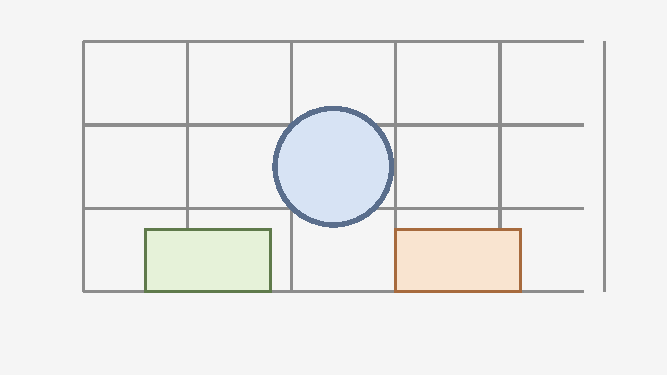
\includegraphics[keepaspectratio]{.gitbook/assets/neutral-grid.pdf}}
\caption{Grid representation of measurement points}
\end{figure}

The figure illustrates how measurement zones can be shown schematically
without naming real locations.

To verify an embedded HTML inlay variant, the following figure can
additionally be used:

\begin{figure}
\centering
\pandocbounded{\includegraphics[keepaspectratio]{.gitbook/assets/ERDA_Logo_simple.png}}
\caption{ERDA logo}
\end{figure}

\newpage

\section{Citations \& further reading}\label{citations-further-reading}

\begin{enumerate}
\def\labelenumi{\arabic{enumi}.}
\tightlist
\item
  \textbf{United Nations Data Portal.} Accessed on 1 June 2024.
  https://data.un.org/
\item
  \textbf{World Bank Open Data.} Accessed on 1 June 2024.
  https://data.worldbank.org/
\item
  \textbf{World Meteorological Organization -- Public Resources.}
  Accessed on 1 June 2024. https://public.wmo.int/en
\item
  \textbf{Smithsonian Open Access.} Accessed on 1 June 2024.
  https://www.si.edu/openaccess
\end{enumerate}

References within the book use numbered footnotes to point consistently
to this list.

\newpage

\# Content note

The content folder now contains complete sample chapters, appendices,
images and templates. Use \hyperref[md-index]{content/index.md} as your
starting point.

\newpage

\# examples

\newpage

\section{Emoji examples -- Activities \&
travel}\label{emoji-examples-activities-travel}

This collection combines sport, hobbies, office workflows and transport
so workflows with combined emojis can be tested.

\subsection{Sport \& fitness}\label{sport-fitness}

\begin{longtable}[]{@{}
  >{\raggedright\arraybackslash}p{(\linewidth - 6\tabcolsep) * \real{0.2500}}
  >{\raggedright\arraybackslash}p{(\linewidth - 6\tabcolsep) * \real{0.2500}}
  >{\raggedright\arraybackslash}p{(\linewidth - 6\tabcolsep) * \real{0.2500}}
  >{\raggedright\arraybackslash}p{(\linewidth - 6\tabcolsep) * \real{0.2500}}@{}}
\toprule\noalign{}
\begin{minipage}[b]{\linewidth}\raggedright
Category
\end{minipage} & \begin{minipage}[b]{\linewidth}\raggedright
Emoji
\end{minipage} & \begin{minipage}[b]{\linewidth}\raggedright
Unicode
\end{minipage} & \begin{minipage}[b]{\linewidth}\raggedright
Notes
\end{minipage} \\
\midrule\noalign{}
\endhead
\bottomrule\noalign{}
\endlastfoot
Endurance & \panEmoji{🏃‍♀️} \panEmoji{🏃‍♂️} \panEmoji{🚴‍♀️} \panEmoji{🚴‍♂️}
\panEmoji{🏊‍♀️} \panEmoji{🏊‍♂️} & Person + Variation Selector & Running,
cycling and swimming \\
Team sports & \panEmoji{⚽} \panEmoji{🏀} \panEmoji{🏐} \panEmoji{🏈}
\panEmoji{⚾} \panEmoji{🥎} & U+26BD · U+1F3C0 · U+1F3D0 · U+1F3C8 ·
U+26BE · U+1F94E & Ball games \\
Precision & \panEmoji{🏓} \panEmoji{🏸} \panEmoji{🏑} \panEmoji{🤺}
\panEmoji{🎯} & U+1F3D3 · U+1F3F8 · U+1F3D1 · U+1F93A · U+1F3AF & Racket
sports, fencing and target practice \\
Winter sports & \panEmoji{⛷️} \panEmoji{🏂} \panEmoji{⛸️} \panEmoji{🛷}
\panEmoji{🥌} & U+26F7 · U+1F3C2 · U+26F8 · U+1F6F7 · U+1F94C & Snow and
ice disciplines \\
Wins & \panEmoji{🏅} \panEmoji{🥇} \panEmoji{🥈} \panEmoji{🥉}
\panEmoji{🏆} & U+1F3C5 · U+1F947 · U+1F948 · U+1F949 · U+1F3C6 &
Awards \\
\end{longtable}

\subsection{Culture \& leisure}\label{culture-leisure}

\begin{longtable}[]{@{}
  >{\raggedright\arraybackslash}p{(\linewidth - 6\tabcolsep) * \real{0.2500}}
  >{\raggedright\arraybackslash}p{(\linewidth - 6\tabcolsep) * \real{0.2500}}
  >{\raggedright\arraybackslash}p{(\linewidth - 6\tabcolsep) * \real{0.2500}}
  >{\raggedright\arraybackslash}p{(\linewidth - 6\tabcolsep) * \real{0.2500}}@{}}
\toprule\noalign{}
\begin{minipage}[b]{\linewidth}\raggedright
Topic
\end{minipage} & \begin{minipage}[b]{\linewidth}\raggedright
Emoji
\end{minipage} & \begin{minipage}[b]{\linewidth}\raggedright
Unicode
\end{minipage} & \begin{minipage}[b]{\linewidth}\raggedright
Description
\end{minipage} \\
\midrule\noalign{}
\endhead
\bottomrule\noalign{}
\endlastfoot
Music & \panEmoji{🎧} \panEmoji{🎤} \panEmoji{🎸} \panEmoji{🎻}
\panEmoji{🎹} \panEmoji{🥁} & U+1F3A7 · U+1F3A4 · U+1F3B8 · U+1F3BB ·
U+1F3B9 · U+1F941 & Audio and instrument tests \\
Art \& media & \panEmoji{🎨} \panEmoji{🖌️} \panEmoji{🖼️} \panEmoji{🎬}
\panEmoji{🎞️} & U+1F3A8 · U+1F58C · U+1F5BC · U+1F3AC · U+1F39E &
Creative domains \\
Games & \panEmoji{🎮} \panEmoji{♟️} \panEmoji{🎲} \panEmoji{🧩} 🃏 &
U+1F3AE · U+265F · U+1F3B2 · U+1F9E9 · U+1F0CF & Game and puzzle
examples \\
Learning & \panEmoji{📚} \panEmoji{🧪} \panEmoji{🧬} \panEmoji{🧠}
\panEmoji{📐} & U+1F4DA · U+1F9EA · U+1F9EC · U+1F9E0 · U+1F4D0 &
Education and lab content \\
Office & \panEmoji{💻} \panEmoji{🖥️} \panEmoji{🖨️} \panEmoji{📠}
\panEmoji{📸} & U+1F4BB · U+1F5A5 · U+1F5A8 · U+1F4E0 · U+1F4F8 & Remote
and studio workflows \\
\end{longtable}

\subsection{Travel \& infrastructure}\label{travel-infrastructure}

\begin{longtable}[]{@{}
  >{\raggedright\arraybackslash}p{(\linewidth - 6\tabcolsep) * \real{0.2500}}
  >{\raggedright\arraybackslash}p{(\linewidth - 6\tabcolsep) * \real{0.2500}}
  >{\raggedright\arraybackslash}p{(\linewidth - 6\tabcolsep) * \real{0.2500}}
  >{\raggedright\arraybackslash}p{(\linewidth - 6\tabcolsep) * \real{0.2500}}@{}}
\toprule\noalign{}
\begin{minipage}[b]{\linewidth}\raggedright
Category
\end{minipage} & \begin{minipage}[b]{\linewidth}\raggedright
Emoji
\end{minipage} & \begin{minipage}[b]{\linewidth}\raggedright
Unicode
\end{minipage} & \begin{minipage}[b]{\linewidth}\raggedright
Context
\end{minipage} \\
\midrule\noalign{}
\endhead
\bottomrule\noalign{}
\endlastfoot
Road transport & \panEmoji{🚗} \panEmoji{🚙} \panEmoji{🚌} \panEmoji{🚎}
\panEmoji{🚚} \panEmoji{🚛} \panEmoji{🚜} & U+1F697--U+1F69C & Road
vehicles \\
Rail & \panEmoji{🚆} \panEmoji{🚇} \panEmoji{🚈} \panEmoji{🚊}
\panEmoji{🚉} & U+1F686 · U+1F687 · U+1F688 · U+1F68A · U+1F689 & Train
types \\
Aviation & \panEmoji{✈️} \panEmoji{🛫} \panEmoji{🛬} \panEmoji{🚁}
\panEmoji{🛩️} & U+2708 · U+1F6EB · U+1F6EC · U+1F681 · U+1F6E9 & Flight
movements \\
Water & \panEmoji{⛴️} \panEmoji{🚢} \panEmoji{🛳️} \panEmoji{🚤}
\panEmoji{🛶} & U+26F4 · U+1F6A2 · U+1F6F3 · U+1F6A4 · U+1F6F6 & Ships
and leisure boats \\
Infrastructure & \panEmoji{🛣️} \panEmoji{🛤️} \panEmoji{🛫} \panEmoji{🧭}
\panEmoji{🗺️} & U+1F6E3 · U+1F6E4 · U+1F6EB · U+1F9ED · U+1F5FA &
Navigation \\
\end{longtable}

\subsection{Testing notes}\label{testing-notes-1}

\begin{itemize}
\tightlist
\item
  Transport emojis often increase line height; use fixed-height tables
  if you want reproducible layout tests.
\item
  Use multi-column layouts so the Twemoji colour font anti-aliases
  correctly in dense sections.
\item
  Combine sports and travel sections to check interactions between
  person ZWJ sequences and pictograms.
\end{itemize}

\newpage

\section{Emoji examples -- Nature \&
food}\label{emoji-examples-nature-food}

This reference page covers plants, weather events, animals and food. Use
the groups to check colour contrast and line wrapping with multi-colour
glyphs.

\subsection{Weather \& environment}\label{weather-environment}

\begin{longtable}[]{@{}
  >{\raggedright\arraybackslash}p{(\linewidth - 6\tabcolsep) * \real{0.2500}}
  >{\raggedright\arraybackslash}p{(\linewidth - 6\tabcolsep) * \real{0.2500}}
  >{\raggedright\arraybackslash}p{(\linewidth - 6\tabcolsep) * \real{0.2500}}
  >{\raggedright\arraybackslash}p{(\linewidth - 6\tabcolsep) * \real{0.2500}}@{}}
\toprule\noalign{}
\begin{minipage}[b]{\linewidth}\raggedright
Topic
\end{minipage} & \begin{minipage}[b]{\linewidth}\raggedright
Emoji
\end{minipage} & \begin{minipage}[b]{\linewidth}\raggedright
Unicode
\end{minipage} & \begin{minipage}[b]{\linewidth}\raggedright
Description
\end{minipage} \\
\midrule\noalign{}
\endhead
\bottomrule\noalign{}
\endlastfoot
Weather & \panEmoji{☀️} \panEmoji{🌤️} \panEmoji{⛅} \panEmoji{🌧️}
\panEmoji{⛈️} \panEmoji{🌩️} \panEmoji{🌪️} & U+2600 · U+1F324--U+1F32A &
Neutral meteorological symbols \\
Sky & \panEmoji{🌈} \panEmoji{🌙} \panEmoji{⭐} \panEmoji{🌌}
\panEmoji{🌠} & U+1F308 · U+1F319 · U+2B50 · U+1F30C · U+1F320 & Light
and night motifs \\
Earth & \panEmoji{🌍} \panEmoji{🌎} \panEmoji{🌏} \panEmoji{🌐}
\panEmoji{🧭} & U+1F30D · U+1F30E · U+1F30F · U+1F310 · U+1F9ED & Global
representations \\
Plants & \panEmoji{🌱} \panEmoji{🌿} \panEmoji{☘️} \panEmoji{🍀}
\panEmoji{🌳} \panEmoji{🌵} & U+1F331 · U+1F33F · U+2618 · U+1F340 ·
U+1F333 · U+1F335 & Vegetation types \\
Elements & \panEmoji{🔥} \panEmoji{💧} \panEmoji{🪨} \panEmoji{🌀}
\panEmoji{🌫️} & U+1F525 · U+1F4A7 · U+1FAA8 · U+1F300 · U+1F32B & Basic
elements and effects \\
\end{longtable}

\subsection{Animals}\label{animals}

\begin{longtable}[]{@{}
  >{\raggedright\arraybackslash}p{(\linewidth - 6\tabcolsep) * \real{0.2500}}
  >{\raggedright\arraybackslash}p{(\linewidth - 6\tabcolsep) * \real{0.2500}}
  >{\raggedright\arraybackslash}p{(\linewidth - 6\tabcolsep) * \real{0.2500}}
  >{\raggedright\arraybackslash}p{(\linewidth - 6\tabcolsep) * \real{0.2500}}@{}}
\toprule\noalign{}
\begin{minipage}[b]{\linewidth}\raggedright
Category
\end{minipage} & \begin{minipage}[b]{\linewidth}\raggedright
Emoji
\end{minipage} & \begin{minipage}[b]{\linewidth}\raggedright
Unicode
\end{minipage} & \begin{minipage}[b]{\linewidth}\raggedright
Notes
\end{minipage} \\
\midrule\noalign{}
\endhead
\bottomrule\noalign{}
\endlastfoot
Mammals & \panEmoji{🐶} \panEmoji{🐱} \panEmoji{🐭} \panEmoji{🐹}
\panEmoji{🐰} \panEmoji{🦊} \panEmoji{🐻} & U+1F436--U+1F43B & Pets and
woodland animals \\
Birds & \panEmoji{🐦} \panEmoji{🦅} \panEmoji{🐧} \panEmoji{🦜}
\panEmoji{🦢} & U+1F426 · U+1F985 · U+1F427 · U+1F99C · U+1F9A2 & Flying
and water birds \\
Reptiles \& amphibians & \panEmoji{🐢} \panEmoji{🐍} \panEmoji{🦎}
\panEmoji{🐸} & U+1F422 · U+1F40D · U+1F98E · U+1F438 & Terrariums and
natural history motifs \\
Insects & \panEmoji{🐝} \panEmoji{🐞} \panEmoji{🦋} \panEmoji{🐜}
\panEmoji{🦟} & U+1F41D · U+1F41E · U+1F98B · U+1F41C · U+1F99F &
Pollination and biology \\
Marine life & \panEmoji{🐟} \panEmoji{🐠} \panEmoji{🐡} \panEmoji{🐬}
\panEmoji{🐳} \panEmoji{🐙} & U+1F41F · U+1F420 · U+1F421 · U+1F42C ·
U+1F433 · U+1F419 & Aquatic diversity \\
\end{longtable}

\subsection{Food \& drink}\label{food-drink}

\begin{longtable}[]{@{}
  >{\raggedright\arraybackslash}p{(\linewidth - 6\tabcolsep) * \real{0.2500}}
  >{\raggedright\arraybackslash}p{(\linewidth - 6\tabcolsep) * \real{0.2500}}
  >{\raggedright\arraybackslash}p{(\linewidth - 6\tabcolsep) * \real{0.2500}}
  >{\raggedright\arraybackslash}p{(\linewidth - 6\tabcolsep) * \real{0.2500}}@{}}
\toprule\noalign{}
\begin{minipage}[b]{\linewidth}\raggedright
Category
\end{minipage} & \begin{minipage}[b]{\linewidth}\raggedright
Emoji
\end{minipage} & \begin{minipage}[b]{\linewidth}\raggedright
Unicode
\end{minipage} & \begin{minipage}[b]{\linewidth}\raggedright
Description
\end{minipage} \\
\midrule\noalign{}
\endhead
\bottomrule\noalign{}
\endlastfoot
Fruit & \panEmoji{🍎} \panEmoji{🍊} \panEmoji{🍌} \panEmoji{🍇}
\panEmoji{🍓} \panEmoji{🥝} \panEmoji{🍍} & U+1F34E--U+1F34A · U+1F34C ·
U+1F347 · U+1F353 · U+1F34F · U+1F34D & Fruit with clear colours \\
Vegetables & \panEmoji{🥕} \panEmoji{🥦} \panEmoji{🧅} \panEmoji{🧄}
\panEmoji{🌽} \panEmoji{🥔} & U+1F955 · U+1F966 · U+1F9C5 · U+1F9C4 ·
U+1F33D · U+1F954 & Food variety \\
Staples & \panEmoji{🍞} \panEmoji{🥐} \panEmoji{🥨} \panEmoji{🥯}
\panEmoji{🍚} \panEmoji{🍝} & U+1F35E · U+1F950 · U+1F968 · U+1F96F ·
U+1F35A · U+1F35D & Grain and pasta dishes \\
Snacks & \panEmoji{🍿} \panEmoji{🍪} \panEmoji{🍩} \panEmoji{🍰}
\panEmoji{🧁} \panEmoji{🍫} & U+1F37F · U+1F36A · U+1F369 · U+1F370 ·
U+1F9C1 · U+1F36B & Sweet examples \\
Drinks & \panEmoji{☕} \panEmoji{🍵} \panEmoji{🥤} \panEmoji{🧃}
\panEmoji{🍺} \panEmoji{🍷} \panEmoji{🍶} & U+2615 · U+1F375 · U+1F964 ·
U+1F9C3 · U+1F37A · U+1F377 · U+1F376 & Hot and cold drinks \\
\end{longtable}

\subsection{Testing notes}\label{testing-notes-2}

\begin{itemize}
\tightlist
\item
  Combine plant or animal sections with the multilingual text templates
  to test line breaks in other scripts.
\item
  Use dark and light background colours to ensure emoji colour layers
  stack correctly when using the Twemoji colour font.
\item
  Also test print output in greyscale to assess contrast.
\end{itemize}

\newpage

\section{Emoji examples -- Objects, symbols \&
flags}\label{emoji-examples-objects-symbols-flags}

This page covers everyday objects, symbols and international flags and
acts as a supplement to the other emoji example collections.

\subsection{Tools \& devices}\label{tools-devices}

\begin{longtable}[]{@{}
  >{\raggedright\arraybackslash}p{(\linewidth - 6\tabcolsep) * \real{0.2500}}
  >{\raggedright\arraybackslash}p{(\linewidth - 6\tabcolsep) * \real{0.2500}}
  >{\raggedright\arraybackslash}p{(\linewidth - 6\tabcolsep) * \real{0.2500}}
  >{\raggedright\arraybackslash}p{(\linewidth - 6\tabcolsep) * \real{0.2500}}@{}}
\toprule\noalign{}
\begin{minipage}[b]{\linewidth}\raggedright
Category
\end{minipage} & \begin{minipage}[b]{\linewidth}\raggedright
Emoji
\end{minipage} & \begin{minipage}[b]{\linewidth}\raggedright
Unicode
\end{minipage} & \begin{minipage}[b]{\linewidth}\raggedright
Description
\end{minipage} \\
\midrule\noalign{}
\endhead
\bottomrule\noalign{}
\endlastfoot
Workshop & \panEmoji{🛠️} \panEmoji{🔧} \panEmoji{🔩} \panEmoji{⚙️}
\panEmoji{🪛} & U+1F6E0 · U+1F527 · U+1F529 · U+2699 · U+1FA9B &
Mechanical components \\
Laboratory & \panEmoji{🔬} \panEmoji{🔭} \panEmoji{⚗️} \panEmoji{🧪}
\panEmoji{🧫} & U+1F52C · U+1F52D · U+2697 · U+1F9EA · U+1F9EB &
Research and analysis \\
Communication & \panEmoji{📱} \panEmoji{📲} \panEmoji{📞} \panEmoji{📡}
\panEmoji{🛰️} & U+1F4F1 · U+1F4F2 · U+1F4DE · U+1F4E1 · U+1F6F0 & Radio
and satellite symbols \\
Household & \panEmoji{🧹} \panEmoji{🧺} \panEmoji{🧼} \panEmoji{🪣}
\panEmoji{🪟} & U+1F9F9 · U+1F9FA · U+1F9FC · U+1FAA3 · U+1FA9F &
Cleaning and household items \\
Energy & \panEmoji{💡} \panEmoji{🔋} \panEmoji{🔌} \panEmoji{♻️}
\panEmoji{🔦} & U+1F4A1 · U+1F50B · U+1F50C · U+267B · U+1F526 & Power
and sustainability icons \\
\end{longtable}

\subsection{Symbols \& signs}\label{symbols-signs}

\begin{longtable}[]{@{}
  >{\raggedright\arraybackslash}p{(\linewidth - 6\tabcolsep) * \real{0.2500}}
  >{\raggedright\arraybackslash}p{(\linewidth - 6\tabcolsep) * \real{0.2500}}
  >{\raggedright\arraybackslash}p{(\linewidth - 6\tabcolsep) * \real{0.2500}}
  >{\raggedright\arraybackslash}p{(\linewidth - 6\tabcolsep) * \real{0.2500}}@{}}
\toprule\noalign{}
\begin{minipage}[b]{\linewidth}\raggedright
Type
\end{minipage} & \begin{minipage}[b]{\linewidth}\raggedright
Emoji
\end{minipage} & \begin{minipage}[b]{\linewidth}\raggedright
Unicode
\end{minipage} & \begin{minipage}[b]{\linewidth}\raggedright
Meaning
\end{minipage} \\
\midrule\noalign{}
\endhead
\bottomrule\noalign{}
\endlastfoot
Warning & \panEmoji{⚠️} \panEmoji{🚸} \panEmoji{⛔} \panEmoji{🚫}
\panEmoji{❗} \panEmoji{❕} & U+26A0 · U+1F6B8 · U+26D4 · U+1F6AB ·
U+2757 · U+2755 & Safety symbols \\
Navigation & \panEmoji{⛳} \panEmoji{🎯} \panEmoji{🧭} \panEmoji{🧭}
\panEmoji{🗺️} & U+26F3 · U+1F3AF · U+1F9ED · (dup.) · U+1F5FA &
Orientation (including intentional duplication for redundancy tests) \\
Time & \panEmoji{⏱️} \panEmoji{⏲️} \panEmoji{⏰} \panEmoji{🕰️}
\panEmoji{🗓️} & U+23F1 · U+23F2 · U+23F0 · U+1F570 · U+1F5D3 & Timers
and calendars \\
Shapes & ⬛ \panEmoji{🟦} ⬜ \panEmoji{🟥} \panEmoji{🟨} \panEmoji{🟩}
\panEmoji{🟧} & U+2B1B · U+1F7E6 · U+2B1C · U+1F7E5 · U+1F7E8 · U+1F7E9
· U+1F7E7 & Area/shape test \\
Religion & \panEmoji{☮️} \panEmoji{☯️} \panEmoji{✝️} \panEmoji{☪️}
\panEmoji{🕉️} \panEmoji{✡️} & U+262E · U+262F · U+271D · U+262A ·
U+1F549 · U+2721 & Spiritual symbols \\
\end{longtable}

\subsection{Flags}\label{flags}

\begin{longtable}[]{@{}lll@{}}
\toprule\noalign{}
Region & Emoji & Description \\
\midrule\noalign{}
\endhead
\bottomrule\noalign{}
\endlastfoot
Global & \panEmoji{🏳️} \panEmoji{🏴} \panEmoji{🏁} \panEmoji{🏳️‍🌈}
\panEmoji{🏳️‍⚧️} & Base symbols incl.~Pride variants \\
Europe & \panEmoji{🇪🇺} \panEmoji{🇩🇪} \panEmoji{🇫🇷} \panEmoji{🇪🇸}
\panEmoji{🇮🇹} \panEmoji{🇵🇱} \panEmoji{🇸🇪} & EU and country flags \\
Americas & \panEmoji{🇺🇳} \panEmoji{🇺🇸} \panEmoji{🇨🇦} \panEmoji{🇧🇷}
\panEmoji{🇦🇷} \panEmoji{🇨🇱} & United Nations and the Americas \\
Africa & \panEmoji{🇪🇬} \panEmoji{🇳🇬} \panEmoji{🇰🇪} \panEmoji{🇿🇦}
\panEmoji{🇪🇹} & North, West, East and Southern Africa \\
Asia \& Oceania & \panEmoji{🇨🇳} \panEmoji{🇯🇵} \panEmoji{🇰🇷}
\panEmoji{🇮🇳} \panEmoji{🇦🇺} \panEmoji{🇳🇿} & Asia-Pacific states \\
\end{longtable}

\subsection{Testing notes}\label{testing-notes-3}

\begin{itemize}
\tightlist
\item
  Flags are made from regional indicator symbols (RIS); ensure the
  chosen font combines the sequences correctly.
\item
  Verify that tables with symbols and tools render via the
  \textbf{DejaVu} set or another licence-compliant serif/sans solution.
\item
  For coloured emojis, the Twemoji colour font remains recommended. In
  PDF workflows, use \texttt{fonts.yml} as the reference so ZWJ
  sequences are embedded.
\end{itemize}

\newpage

\section{Emoji examples -- Smileys \&
people}\label{emoji-examples-smileys-people}

This page groups commonly used emoji sets by emotions, gestures and role
profiles. It serves as a reference to test layouts, fonts and emoji
fallbacks.

\subsection{Smileys \& emotions}\label{smileys-emotions}

\begin{longtable}[]{@{}
  >{\raggedright\arraybackslash}p{(\linewidth - 6\tabcolsep) * \real{0.2500}}
  >{\raggedright\arraybackslash}p{(\linewidth - 6\tabcolsep) * \real{0.2500}}
  >{\raggedright\arraybackslash}p{(\linewidth - 6\tabcolsep) * \real{0.2500}}
  >{\raggedright\arraybackslash}p{(\linewidth - 6\tabcolsep) * \real{0.2500}}@{}}
\toprule\noalign{}
\begin{minipage}[b]{\linewidth}\raggedright
Category
\end{minipage} & \begin{minipage}[b]{\linewidth}\raggedright
Emoji
\end{minipage} & \begin{minipage}[b]{\linewidth}\raggedright
Unicode
\end{minipage} & \begin{minipage}[b]{\linewidth}\raggedright
Description
\end{minipage} \\
\midrule\noalign{}
\endhead
\bottomrule\noalign{}
\endlastfoot
Happy & \panEmoji{😀} \panEmoji{😃} \panEmoji{😄} \panEmoji{😁}
\panEmoji{😆} \panEmoji{😅} & U+1F600--U+1F606 & Standard smileys for
positive reactions \\
Affectionate & \panEmoji{😊} \panEmoji{🥰} \panEmoji{😍} \panEmoji{😘}
\panEmoji{😻} & U+1F60A · U+1F970 · U+1F60D · U+1F618 · U+1F63B & Warm
reactions and animal variants \\
Surprise & \panEmoji{🤩} \panEmoji{😮} \panEmoji{😯} \panEmoji{😲}
\panEmoji{🥳} & U+1F929 · U+1F62E · U+1F62F · U+1F632 · U+1F973 &
Astonishment and party mood \\
Thoughtful & \panEmoji{🤔} \panEmoji{😐} \panEmoji{😑} \panEmoji{😶}
\panEmoji{🤨} & U+1F914 · U+1F610 · U+1F611 · U+1F636 · U+1F928 &
Neutral or sceptical faces \\
Stress & \panEmoji{😰} \panEmoji{😱} \panEmoji{😨} \panEmoji{😢}
\panEmoji{😭} & U+1F630 · U+1F631 · U+1F628 · U+1F622 · U+1F62D &
Stress, worry and sadness \\
Health & \panEmoji{🤒} \panEmoji{🤕} \panEmoji{🤧} \panEmoji{😷}
\panEmoji{😴} & U+1F912 · U+1F915 · U+1F927 · U+1F637 · U+1F634 &
Medical emojis and sleep \\
\end{longtable}

\subsection{Gestures \& hands}\label{gestures-hands}

\begin{longtable}[]{@{}
  >{\raggedright\arraybackslash}p{(\linewidth - 6\tabcolsep) * \real{0.2500}}
  >{\raggedright\arraybackslash}p{(\linewidth - 6\tabcolsep) * \real{0.2500}}
  >{\raggedright\arraybackslash}p{(\linewidth - 6\tabcolsep) * \real{0.2500}}
  >{\raggedright\arraybackslash}p{(\linewidth - 6\tabcolsep) * \real{0.2500}}@{}}
\toprule\noalign{}
\begin{minipage}[b]{\linewidth}\raggedright
Type
\end{minipage} & \begin{minipage}[b]{\linewidth}\raggedright
Emoji
\end{minipage} & \begin{minipage}[b]{\linewidth}\raggedright
Unicode
\end{minipage} & \begin{minipage}[b]{\linewidth}\raggedright
Purpose
\end{minipage} \\
\midrule\noalign{}
\endhead
\bottomrule\noalign{}
\endlastfoot
Approval & \panEmoji{👍} \panEmoji{👏} \panEmoji{🤝} \panEmoji{🙌} &
U+1F44D · U+1F44F · U+1F91D · U+1F64C & Approval and co-operation \\
Refusal & \panEmoji{👎} \panEmoji{🙅} \panEmoji{🙅‍♂️} \panEmoji{🙅‍♀️} &
U+1F44E · U+1F645 · ZWJ sequences & Negation and stopping \\
Pointers & \panEmoji{☝️} \panEmoji{✍️} \panEmoji{👉} \panEmoji{👈}
\panEmoji{👆} \panEmoji{👇} & U+261D · U+270D · U+1F449 · U+1F448 ·
U+1F446 · U+1F447 & Pointing gestures \\
Culture & \panEmoji{🤲} \panEmoji{👐} \panEmoji{🤘} \panEmoji{🤙}
\panEmoji{🤟} & U+1F932 · U+1F450 · U+1F918 · U+1F919 · U+1F91F &
Greetings and music gestures \\
Inclusive & \panEmoji{✋} \panEmoji{✋🏻} \panEmoji{✋🏽} \panEmoji{✋🏿} &
U+270B + Fitzpatrick modifiers & Skin tones for accessibility \\
\end{longtable}

\subsection{People \& roles}\label{people-roles}

\begin{longtable}[]{@{}
  >{\raggedright\arraybackslash}p{(\linewidth - 6\tabcolsep) * \real{0.2500}}
  >{\raggedright\arraybackslash}p{(\linewidth - 6\tabcolsep) * \real{0.2500}}
  >{\raggedright\arraybackslash}p{(\linewidth - 6\tabcolsep) * \real{0.2500}}
  >{\raggedright\arraybackslash}p{(\linewidth - 6\tabcolsep) * \real{0.2500}}@{}}
\toprule\noalign{}
\begin{minipage}[b]{\linewidth}\raggedright
Category
\end{minipage} & \begin{minipage}[b]{\linewidth}\raggedright
Emoji
\end{minipage} & \begin{minipage}[b]{\linewidth}\raggedright
Unicode
\end{minipage} & \begin{minipage}[b]{\linewidth}\raggedright
Description
\end{minipage} \\
\midrule\noalign{}
\endhead
\bottomrule\noalign{}
\endlastfoot
Everyday & \panEmoji{🙂} \panEmoji{🧑‍🦰} \panEmoji{🧑‍🦱} \panEmoji{🧑‍🦳} &
Standard face and hair variants & Facial features with neutral
colours \\
Occupation & \panEmoji{👩‍💻} \panEmoji{👨‍🔧} \panEmoji{🧑‍🏫} \panEmoji{🧑‍🌾} &
ZWJ sequences & Professional depictions \\
Family & \panEmoji{👨‍👩‍👧} \panEmoji{👩‍👧‍👦} \panEmoji{👨‍👨‍👧‍👦} & Family ZWJ &
Diversity in households \\
Emergency/services & \panEmoji{👩‍🚒} \panEmoji{👮‍♂️} \panEmoji{🧑‍🚀}
\panEmoji{🧑‍⚕️} & ZWJ sequences & Uniforms and services \\
Diversity & \panEmoji{🧕} \panEmoji{🧔‍♂️} \panEmoji{🧑‍🦽} \panEmoji{🧑‍🦯} &
U+1F93F etc. & Cultural and assistance examples \\
\end{longtable}

\subsection{Testing notes}\label{testing-notes-4}

\begin{itemize}
\tightlist
\item
  Combine these emoji rows with text blocks in different scripts to
  check interactions with line heights.
\item
  For coloured glyphs, embedding the \textbf{Twemoji Color Font} is
  recommended; for monochrome tests, Twemoji can be rendered in
  greyscale.
\item
  Add additional emojis with ZWJ or skin tone modifiers if your
  workflows require it.
\end{itemize}

\newpage

\section{Preface}\label{preface}

This preface explains the purpose and structure of the sample book. All
content is deliberately phrased in a neutral way so it can be used for
usability tests, layout demos and localisation workflows.

\begin{itemize}
\tightlist
\item
  \textbf{Audience:} teams who want to test text, image or table
  components without using real customer data.
\item
  \textbf{Structure:} each section contains at least one element
  commonly found in book production -- for example figures,
  cross-references, citations or tables.
\item
  \textbf{International scope:} the included template for multilingual
  text covers common major languages and can be extended.
\end{itemize}

Further guidance can be found in
\hyperref[md-chapters-chapter-01]{Chapter 1}, while
\hyperref[md-chapters-chapter-02]{Chapter 2} provides concrete table
layouts.

\newpage

\# templates

\newpage

\section{Template for multilingual neutral
text}\label{template-for-multilingual-neutral-text}

The following structure shows how neutral text building blocks can be
written in multiple languages. Use short sentences, avoid personal
details, and avoid culture- or brand-specific terms.

\subsection{Basic structure}\label{basic-structure}

\begin{verbatim}
## Context
Short description of the scenario.

### Language (ISO code)
Neutral paragraph.
\end{verbatim}

\subsection{Example: global weather
observation}\label{example-global-weather-observation}

\begin{itemize}
\tightlist
\item
  \textbf{Context:} a team describes a calm day with moderate weather
  readings.
\end{itemize}

\subsubsection{German (de)}\label{german-de}

Ein moderater Morgen brachte gleichmäßige Temperaturen, wodurch
Messgeräte ohne Anpassung betrieben werden konnten.

\subsubsection{English (en)}\label{english-en}

The observation team noted a calm day with stable readings, enabling
straightforward comparisons over the week.

\subsubsection{French (fr)}\label{french-fr}

L'équipe a enregistré une journée stable, ce qui facilite la comparaison
avec les mesures précédentes.

\subsubsection{Spanish (es)}\label{spanish-es}

El equipo observó un día sereno con datos regulares que permiten revisar
tendencias sin sesgos.

\subsubsection{Portuguese (pt)}\label{portuguese-pt}

A equipe registrou um período estável, adequado para validar calibragens
e rotinas de manutenção.

\subsubsection{Italian (it)}\label{italian-it}

Il gruppo ha descritto una giornata equilibrata, utile per mantenere le
serie temporali coerenti.

\subsubsection{Dutch (nl)}\label{dutch-nl}

Het team rapporteerde een rustige dag met meetwaarden die zonder
correcties konden worden vastgelegd.

\subsubsection{Bulgarian (bg)}\label{bulgarian-bg}

Екипът отбеляза спокоен ден с равномерни данни, което улеснява
сравненията в рамките на седмицата.

\subsubsection{Croatian (hr)}\label{croatian-hr}

Tim je zabilježio miran dan s ujednačenim vrijednostima koje
pojednostavljuju usporedbe tijekom tjedna.

\subsubsection{Czech (cs)}\label{czech-cs}

Tým zaznamenal klidný den se stabilními hodnotami, takže týdenní
porovnání probíhá bez úprav.

\subsubsection{Danish (da)}\label{danish-da}

Holdet noterede en rolig dag med jævne målinger, hvilket gør det let at
sammenligne ugens værdier.

\subsubsection{Estonian (et)}\label{estonian-et}

Meeskond kirjeldas rahulikku päeva ühtlaste näitudega, mis hõlbustab
nädalate võrdlemist.

\subsubsection{Finnish (fi)}\label{finnish-fi}

Tiimi mukaan päivä oli tasainen ja mittaukset pysyivät muuttumattomina,
mikä tukee vertailevaa seurantaa.

\subsubsection{Greek (el)}\label{greek-el}

Η ομάδα κατέγραψε ήρεμη ημέρα με σταθερές μετρήσεις που διευκολύνουν τις
εβδομαδιαίες συγκρίσεις.

\subsubsection{Hungarian (hu)}\label{hungarian-hu}

A csapat nyugodt napot írt le, amelynek mérései stabilak maradtak, így
könnyű a heti összevetés.

\subsubsection{Irish (ga)}\label{irish-ga}

Luaigh an fhoireann lá ciúin le léamha cobhsaí a éascaíonn comparáidí
seachtainiúla.

\subsubsection{Latvian (lv)}\label{latvian-lv}

Komanda aprakstīja mierīgu dienu ar vienmērīgiem rādījumiem, kas
atvieglo salīdzināšanu nedēļas griezumā.

\subsubsection{Lithuanian (lt)}\label{lithuanian-lt}

Komanda užfiksavo ramią dieną su stabiliais duomenimis, todėl
savaitiniai palyginimai yra paprasti.

\subsubsection{Maltese (mt)}\label{maltese-mt}

It-tim irreġistra ġurnata kwieta b'qari stabbli li jagħmlu aktar faċli
li tqabbel id-dejta tal-ġimgħa.

\subsubsection{Polish (pl)}\label{polish-pl}

Zespół odnotował spokojny dzień ze stałymi odczytami, co ułatwia
porównania tygodniowe.

\subsubsection{Romanian (ro)}\label{romanian-ro}

Echipa a remarcat o zi calmă cu valori stabile, ușurând comparațiile din
cursul săptămânii.

\subsubsection{Slovak (sk)}\label{slovak-sk}

Tím opísal pokojný deň so stabilnými údajmi, ktoré pomáhajú pri
porovnávaní v rámci týždňa.

\subsubsection{Slovenian (sl)}\label{slovenian-sl}

Ekipa je opisala miren dan z enakomernimi meritvami, kar olajša tedenske
primerjave.

\subsubsection{Swedish (sv)}\label{swedish-sv}

Teamet noterade en lugn dag med stabila värden som gör jämförelser under
veckan enklare.

\subsubsection{Ukrainian (uk)}\label{ukrainian-uk}

Команда спостерігала спокійний день зі стабільними показниками, що
спрощує тижневі порівняння.

\subsubsection{Arabic (ar)}\label{arabic-ar}

سجل الفريق يوماً هادئاً بقراءات مستقرة تسهّل مقارنة البيانات خلال الأسبوع.

\subsubsection{Chinese (zh)}\label{chinese-zh}

观测团队记录了一个稳定的日子,数据平稳,有助于持续对比不同周的趋势。

\subsubsection{Japanese (ja)}\label{japanese-ja}

観測チームは穏やかな一日を記録し、安定したデータが週次比較を容易にすると述べました。

\subsubsection{Korean (ko)}\label{korean-ko}

관측 팀은 측정값이 고르게 유지된 차분한 하루를 기록하여 주간 비교가
수월해졌다고 보고했습니다.

\subsubsection{Hindi (hi)}\label{hindi-hi}

टीम ने एक शांत दिन दर्ज किया जहाँ मान स्थिर रहे और साप्ताहिक तुलना सरल हो गई।

\subsubsection{Indonesian (id)}\label{indonesian-id}

Tim melaporkan hari tenang dengan bacaan stabil sehingga peninjauan
mingguan dapat dilakukan tanpa penyesuaian.

\subsubsection{Filipino (fil)}\label{filipino-fil}

Iniulat ng koponan ang isang mahinahong araw na may pantay na datos,
kaya mas madali ang paghahambing ng lingguhan.

\subsubsection{Māori (mi)}\label{mux101ori-mi}

I tuhi te rōpū tirotiro i tētahi rā mārie me ngā uara tōtika, he mea
māmā ai te whakataurite ā-wiki.

\subsubsection{Samoan (sm)}\label{samoan-sm}

Na fa'amau e le 'au se aso filemu ma faitauga toniga e faafaigofie ai
su'esu'ega o vaiaso ta'itasi.

\subsubsection{Swahili (sw)}\label{swahili-sw}

Timu ilieleza siku tulivu yenye takwimu thabiti zinazorahisisha
kulinganisha kwa wiki.

\subsubsection{Amharic (am)}\label{amharic-am}

ቡድኑ በተመጣጣኝ መዝገቦች ያለ የተረጋጋ ቀን መመዝገቡን አግልፆ እርምጃዎችን ለአስተካክል ቀላል እንደሚያደርግ
ገለጸ።

\subsubsection{Yoruba (yo)}\label{yoruba-yo}

Ẹgbẹ́ náà sọ pé ọjọ́ naa dakẹ́ nígbà tí àwọ́n ìwọn ṣetán bí wọ́n ṣe rí, kí
iṣirò ọ̀sẹ̀ rọrùn.

\subsubsection{Hausa (ha)}\label{hausa-ha}

Ƙungiyar ta lura da ranar natsuwa mai daidaitattun bayanai da ke sauƙaƙa
kwatancen mako-mako.

\subsubsection{Inuktitut (iu)}\label{inuktitut-iu}

ᐊᒥᓱᓂ ᐱᒋᐊᕐᔪᖅ ᐅᑭᐅᑎᖅ ᐃᒡᓗᓕᖅ ᑐᙵᓇᐅᑎᓪᓗᓂ ᐱᖃᓗᒍ ᐅᓇ ᐃᓄᖅᑐᐊᓕᕐᓂᖅ ᑐᓴᖅᑕᐅᔪᒥ.

\subsubsection{Turkish (tr)}\label{turkish-tr}

Ekip, ölçümlerin dengede kaldığı sakin bir gün bildirerek haftalık
karşılaştırmaların kolaylaştığını belirtti.

\subsubsection{Azerbaijani (az)}\label{azerbaijani-az}

Komanda sabit göstəricilərlə sakit bir gün qeydə aldı və bu da həftəlik
müqayisələri sadələşdirir.

\subsubsection{Kazakh (kk)}\label{kazakh-kk}

Топ тұрақты көрсеткіштер сақталған тыныш күнді сипаттап, апталық
салыстыруды жеңілдететінін айтты.

This list can be extended as needed. Add notes on writing systems or
reading direction where relevant (for example for Arabic or Hebrew).

\end{document}
